\section{Experimental Results}
\label{sec:experimentalResults}

\subsection{Curriculum Learning with Aerial Imagery}
\label{sec:results_curriculum_learning_aerial_imagery}

\begin{figure}[!h]
\begin{subfigure}{0.48\textwidth}
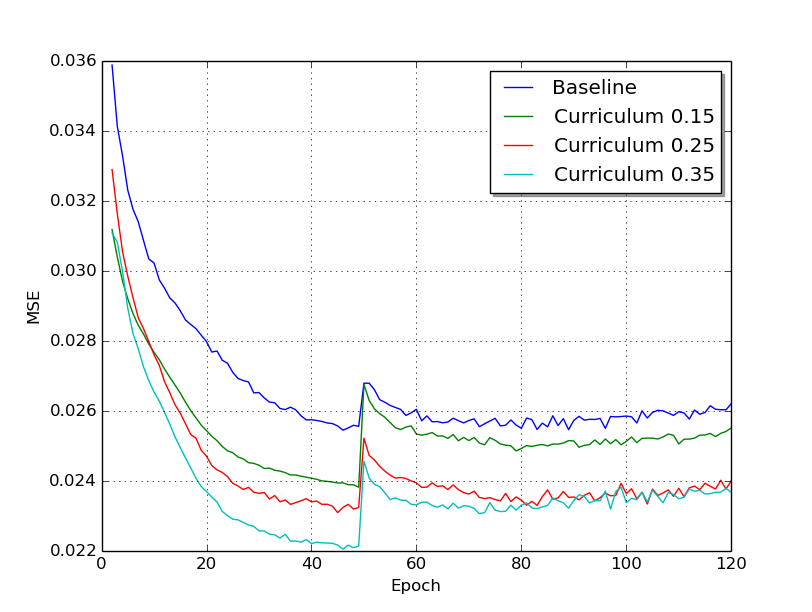
\includegraphics[width=\linewidth]{figs/E1/E1-lc.png}
\caption{Comparison of test loss} \label{fig:E1_curr_norway_loss}
\end{subfigure}
\hspace*{\fill} % separation between the subfigures
\begin{subfigure}{0.48\textwidth}
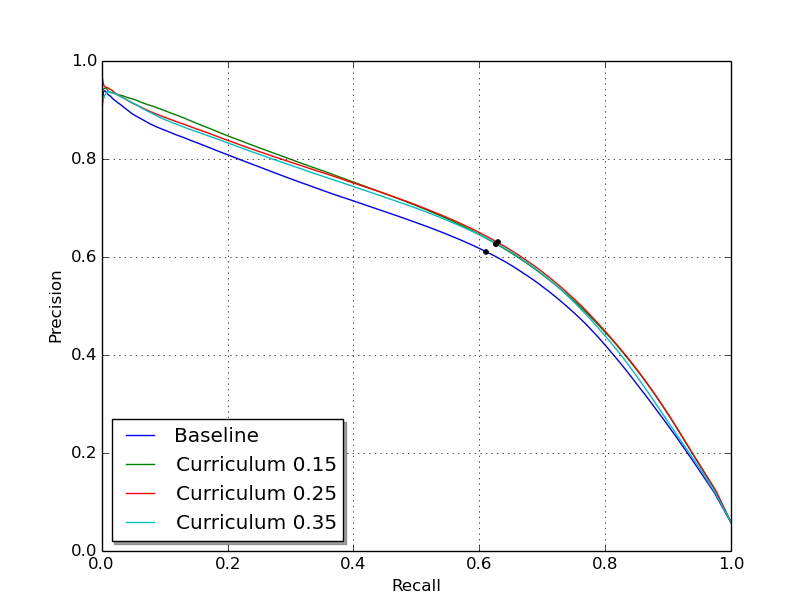
\includegraphics[width=\linewidth]{figs/E1/E1-pr.png}
\caption{Precision and recall comparisons.} \label{fig:E1_curr_norway_pr}
\end{subfigure}
\hspace*{\fill} % separation between the subfigures
\caption{E1 - Performance of curriculum learning at different thresholds, $D_{0}$ for Norwegian Roads Dataset Vbase} \label{fig:E1_curriculum_norway}
\end{figure}

In Experiment E1, the road detection system was trained on four different patch datasets. The system's performance for each of these datasets are displayed in Figure \ref{fig:E1_curriculum_norway}. A comparison of the test loss per epoch is displayed in Figure \ref{fig:E1_curr_norway_loss}, whereas the final performance of each patch dataset is shown by a precision and recall curve in Figure \ref{fig:E1_curr_norway_pr}. The network configuration used for the tests was identical, as well as the number of training examples seen during training. Essentially, the performance gap between the baseline and curriculum plots, comes from the first stage of the patch datasets, where different difficulty threshold $D_0$ have been used.\\

Observing the plots in Figure \ref{fig:E1_curr_norway_loss}, the switch between stage 0 and stage 1, is clearly visible at epoch 50. The increase in test loss is most severe in the datasets formed by a curriculum strategy. Leading up to epoch 50, the curriculum plots show an increasing gap in test performance, if compared to the baseline plot. After the switch the curriculum datasets still outperform the baseline dataset, even though the training set distribution of stage 1 are the same for all patch datasets.\\

Furthermore, the networks trained with a curriculum strategy shows an improved precision for all levels of recall compared to the baseline.\\

An interesting trend between the thresholds $D_0$ and the loss, is that decreasing the difficulty threshold, does not necessarily produce better results. The patch dataset \textit{Curriculum 0.15} has the easiest first stage, yet performed worse than \textit{Curriculum 0.25} and \textit{Curriculum 0.35}. \\

%A similar experiment was also performed on the Massachusetts Roads Dataset. In Experiment E2, networks are trained with three different patch datasets. The baseline dataset's first stage has a distribution similar to the aerial image dataset's training set. The curriculum dataset has a difficulty threshold $D_0$ of 0.25, which exclude every example with a estimated difficulty above 0.25 from the first stage. In contrast, the anti-curriculum patch dataset only include road patch examples with a difficulty above 0.25. The curriculum teacher model is really good at predicting patches that contain no road label pixels, there are very few non-road patches with a difficulty rating above 0.25. This is why the anti-curriculum's first stage does not exclude any non-road patches \todo{A bit weirdy spoken}. \\


The results from experiment  E2 can be seen in Figure \ref{fig:E2_curriculum_mass}. This experiment was conducted using the Massachusetts Roads Dataset. The switch from stage 0 and stage 1 is visible for the \textit{Baseline} and \textit{Anti-curriculum} loss plots at epoch 50. A network trained with the curriculum patch dataset, performed better than the baseline as seen in Figure \ref{fig:E2_curr_mass_loss} and Figure \ref{fig:E2_curr_mass_pr}. Training with an anti-curriculum strategy, where the first stage consists of harder examples, does not provide the same loss, or breakeven performance. This is especially evident in the test loss plot, where the network converge at around epoch 25, and starts to overfit towards epoch 50. From epoch 50 when stage 1 examples entered the training set, there is a dramatic decrease in test loss. The test loss decrease continues at a steady pace until epoch 85. Yet, the final performance of anti-curriculum learning is substantially lower than both the baseline and curriculum learning, as illustrated by the breakeven points in Figure \ref{fig:E2_curr_mass_pr}.\\

The precision and recall breakeven values from Experiment E1 and Experiment E2, are listed in Table \ref{tab:results_curriculum_learning_breakeven}, and shows that training with a curriculum strategy was beneficial for both datasets.\\
\begin{figure}
\begin{subfigure}{0.48\textwidth}
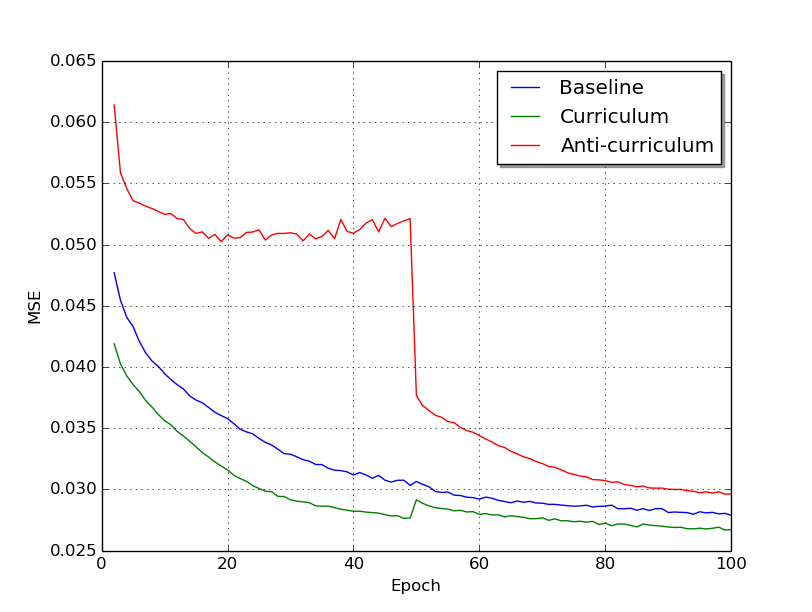
\includegraphics[width=\linewidth]{figs/E2/E2-lc.png}
\caption{Comparison of test loss} \label{fig:E2_curr_mass_loss}
\end{subfigure}
\hspace*{\fill} % separation between the subfigures
\begin{subfigure}{0.48\textwidth}
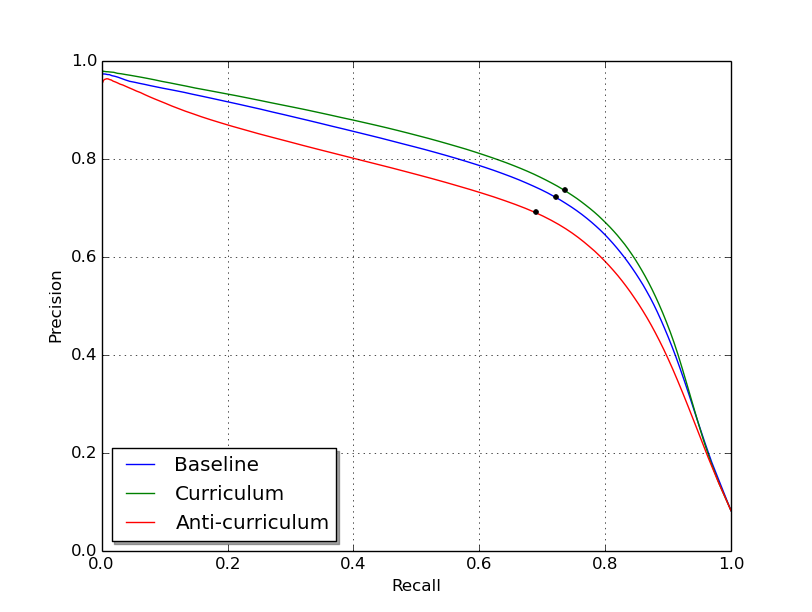
\includegraphics[width=\linewidth]{figs/E2/E2-pr.png}
\caption{Precision and recall comparisons.} \label{fig:E2_curr_mass_pr}
\end{subfigure}
\hspace*{\fill} % separation between the subfigures
\caption{E2 - Performance of curriculum learning and anti-curriculum learning for Massachusetts Roads Dataset} \label{fig:E2_curriculum_mass}
\end{figure}

\begin{table}
\caption{Curriculum learning results.}
\begin{center}
\begin{adjustbox}{max width=\textwidth}
\begin{tabular}{+l ^l ^l ^r}\hline
\rowstyle{\bfseries}
  Experiment & $\mathbf{D_0}$ & Dataset & Breakeven\\\hline
  Baseline & 1.0 & Norwegian & 0.6105 \\
  Curriculum &0.15 & Norwegian & 0.6264 \\
  Curriculum &0.25 & Norwegian & \textbf{0.6292} \\
  Curriculum &0.35 & Norwegian & 0.6269 \\\hline
  Baseline &1.0& Massachusetts & 0.7211 \\
  Curriculum &0.25& Massachusetts & 0.\textbf{7353} \\
  Anti-curriculum &0.25 & Massachusetts & 0.6904 \\\hline
\end{tabular}
\end{adjustbox}
\end{center}
\label{tab:results_curriculum_learning_breakeven}
\end{table}

The training set difficulty distribution, according to the difficulty estimator $d(y,q)$ used with the curriculum teacher model from in Experiment E2\todo{Wierd sentence}, is depicted in a histogram in Figure \ref{fig:E2_difficulty_distribution}. The training set of  Massachusetts Roads Dataset was sampled, and the difficulty estimate for each patch was computed for every patch. The patches which contain no road label pixels, were counted separately from patches containing road label pixels. The resulting histogram for non-road patches in Figure \ref{fig:E2_difficulty_distribution_nonroad}, shows that the trained curriculum model is excellent at predicting non-road patches, because the predictions and labels match very well resulting in very low difficulty estimates. This is not the case for road patches, illustrated by Figure  \ref{fig:E2_difficulty_distribution_road}, where the distribution is clearly skewed right and have a greater variance. \\

\begin{figure}
\begin{subfigure}{0.48\textwidth}
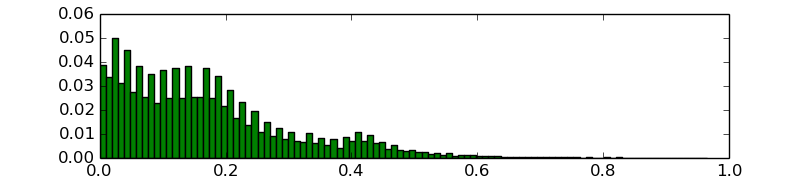
\includegraphics[width=\linewidth]{figs/E2/E2-road-dist.png}
\caption{Distribution for road patches.} \label{fig:E2_difficulty_distribution_road}
\end{subfigure}
\hspace*{\fill} % separation between the subfigures
\begin{subfigure}{0.48\textwidth}
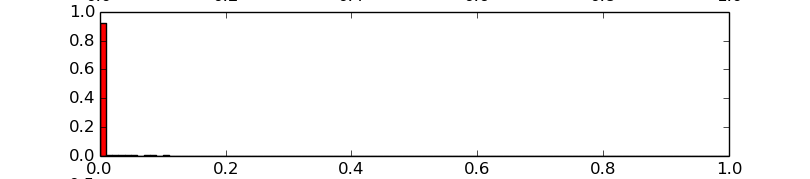
\includegraphics[width=\linewidth]{figs/E2/E2-non_road-dist.png}
\caption{Distribution for non-road patches.} \label{fig:E2_difficulty_distribution_nonroad}
\end{subfigure}
\hspace*{\fill} % separation between the subfigures
\caption{E2 - Example difficulty distribution according to estimator $d(y,q)$ } \label{fig:E2_difficulty_distribution}
\end{figure}

Figure \ref{fig:E7_curriculum_inexperienced} shows the results from Experiment E7. The patch datasets in this experiment were created from a teacher that was trained with the same number of training examples as the patch datasets \todo{Double patch datasets in sentence}. Curriculum learning still achieves a higher test loss and a gives better precision for all levels of recall. In addition to comparing the baseline and curriculum learning which have two stages, Figure \ref{fig:E7_curriculum_inexperienced_loss} and \ref{fig:E7_curriculum_inexperienced_pr} illustrate the performance of training with only the first stage of the patch datasets. As expected, the first stage baseline has a lower breakeven point than the two stage baseline. More surprisingly, the first stage curriculum outperformed both the baseline and the curriculum, both in terms of breakeven and test loss. However, at recall levels less than 0.4, the precision of the first stage curriculum decreases rapidly. This shows that the curriculum strategy is effective at filtering out inconsistent labels, and with a suitable difficulty threshold $D_0$ can provides enough example variability in the first stage training set. Another possible reason for this result, is the sudden training set switch at epoch 60, which dramatically increases the test loss. \\

\begin{figure}
\begin{subfigure}{0.48\textwidth}
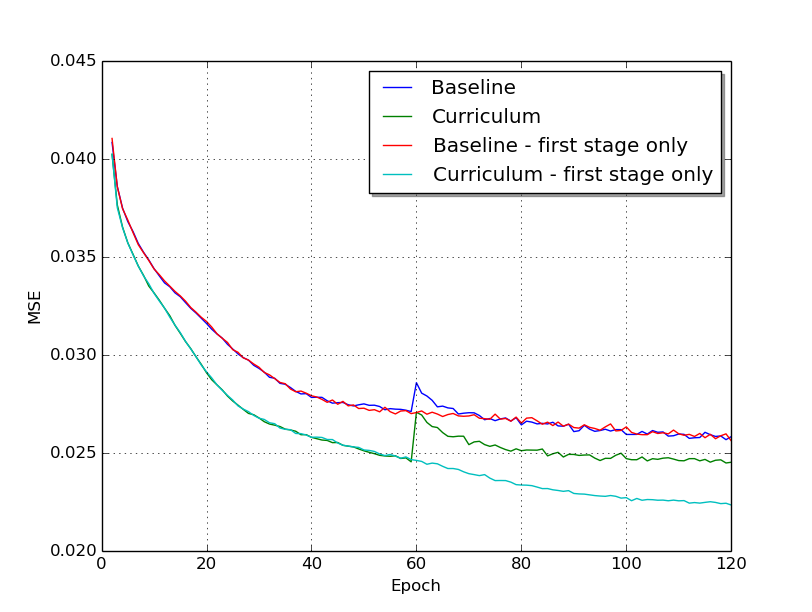
\includegraphics[width=\linewidth]{figs/E7/E7_lc_two_stage.png}
\caption{Test loss for two stage dataset} \label{fig:E7_curriculum_inexperienced_loss}
\end{subfigure}
\hspace*{\fill} % separation between the subfigures
\begin{subfigure}{0.48\textwidth}
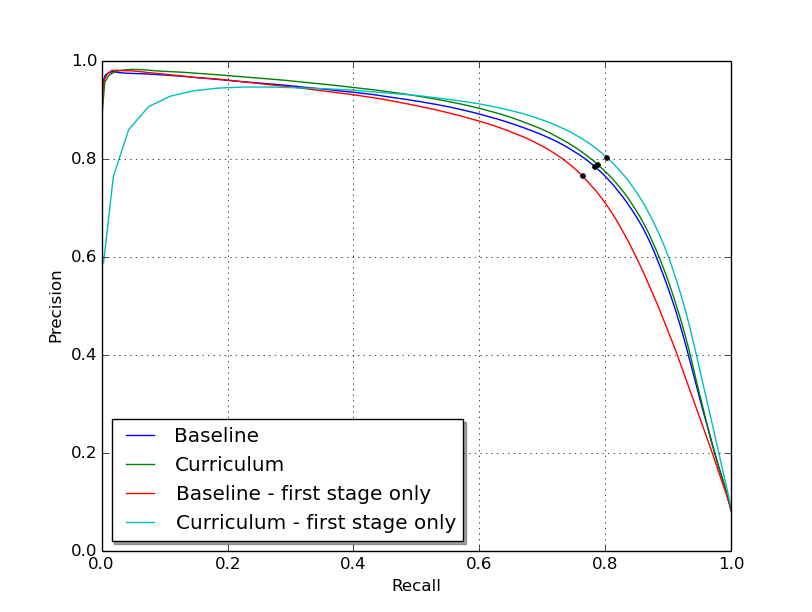
\includegraphics[width=\linewidth]{figs/E7/E7_pr_two_stage.png}
\caption{Precision and recall comparisons for two stage dataset.} \label{fig:E7_curriculum_inexperienced_pr}
\end{subfigure}

\begin{subfigure}{0.48\textwidth}
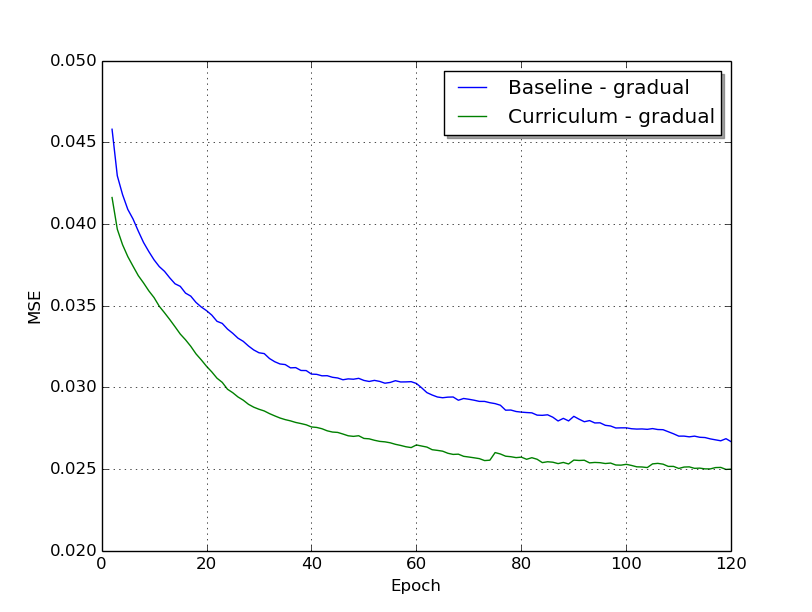
\includegraphics[width=\linewidth]{figs/E7/E7_lc_gradual.png}
\caption{Test loss for dataset with gradual stage switching} \label{fig:E7_gradual_loss}
\end{subfigure}
\hspace*{\fill} % separation between the subfigures
\begin{subfigure}{0.48\textwidth}
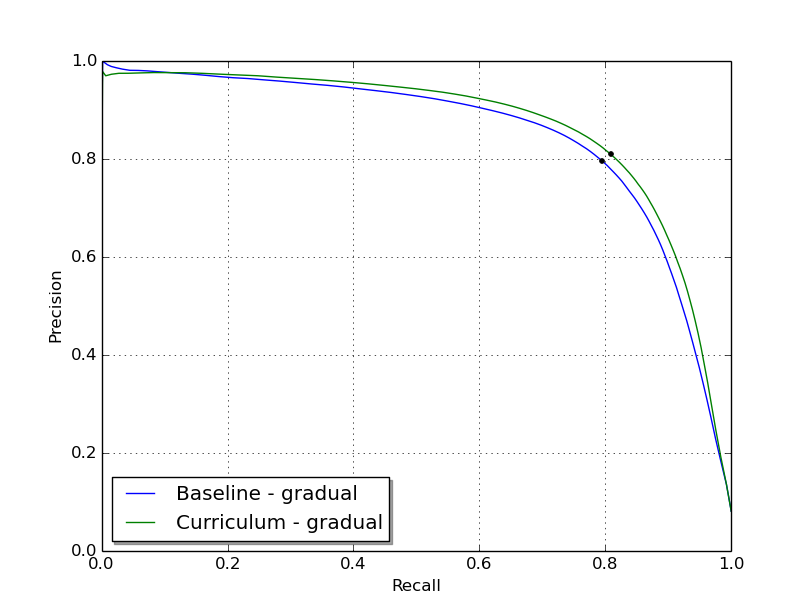
\includegraphics[width=\linewidth]{figs/E7/E7_pr_gradual.png}
\caption{Precision and recall for dataset with gradual stage switching.} \label{fig:E7_gradual_pr}
\end{subfigure}
\hspace*{\fill} % separation between the subfigures
\caption{E7 - Results from Experiment E7.} \label{fig:E7_curriculum_inexperienced}
\end{figure}

This was further explored by creating two additional patch datasets, with 5 stages each. The first stage has 108000 examples, while the other 4 stages contain 54000 examples each. Subsequent stages replaces the training set, by assigning each example to a random position in the training set. Because the positions are picked by random sampling with replacement, only around 40\% of the existing examples in the training set are replaced at each switch. This results in a more gradual transition of the difficulty distribution. In Figure \ref{fig:E7_gradual_loss}, the stage switching with these patch datasets, results in the test loss being more stable.
The baseline plot even decreases substantially after epoch 60. This is an improvement from the spiking behaviour from the two stage baseline. The gradual approach also shows promise in Figure \ref{fig:E7_curriculum_inexperienced}, where the curriculum plot achieves a breakeven point of 0.809, compared to the breakeven of 0.802 for the first stage curriculum. The gradual baseline approach only achieved a breakeven of 0.795.\\

\subsection{Bootstrapping for Imagery with Noisy Labels}
\label{sec:results_bootstrapping}

The results from comparing the bootstrapping methods and the baseline method at several levels of label noise, are displayed in Figure \ref{fig:E3_boot_mass} and Figure \ref{fig:E5_boot_norway}. The plots in the first figure are based on models trained on the Massachusetts Roads Dataset, whereas the second figure show results from training on the Norwegian Roads Dataset. Label noise have been artificially added to the label images before training. Specifically, areas of road pixels have been removed incrementally, by setting the label pixel values to zero. This process is continued until a certain percentage of road class pixels have been removed. In terms of aerial imagery, the artificially added label noise simulates omission errors, in which roads have not been marked in the label maps. Experiment E3 and E5, utilized patch datasets where 0, 10, 20 ,30 and 40 percent of roads were removed from the labels \todo{Example of road removal}.\\

\begin{figure}
\begin{subfigure}{0.48\textwidth}
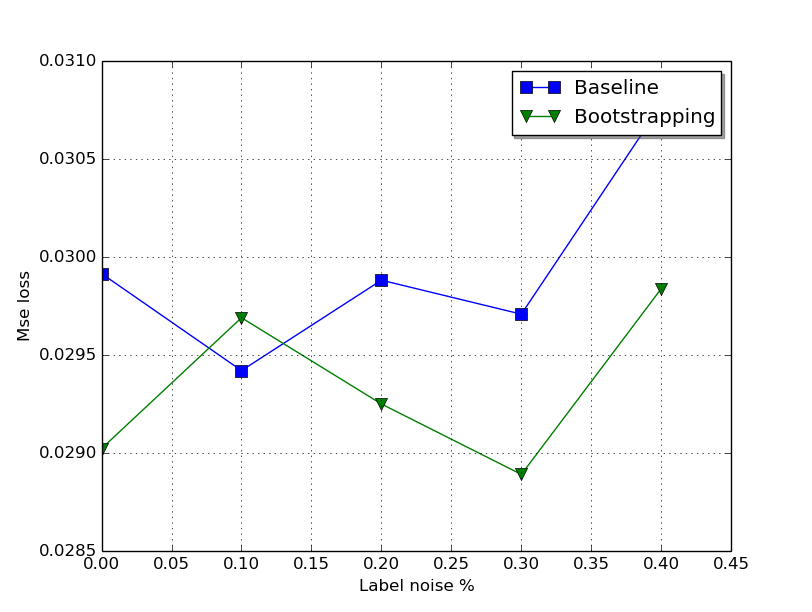
\includegraphics[width=\linewidth]{figs/E3/E3_lc_noise.png}
\caption{MSE test loss} \label{fig:E3_boot_mass_loss}
\end{subfigure}
\hspace*{\fill} % separation between the subfigures
\begin{subfigure}{0.48\textwidth}
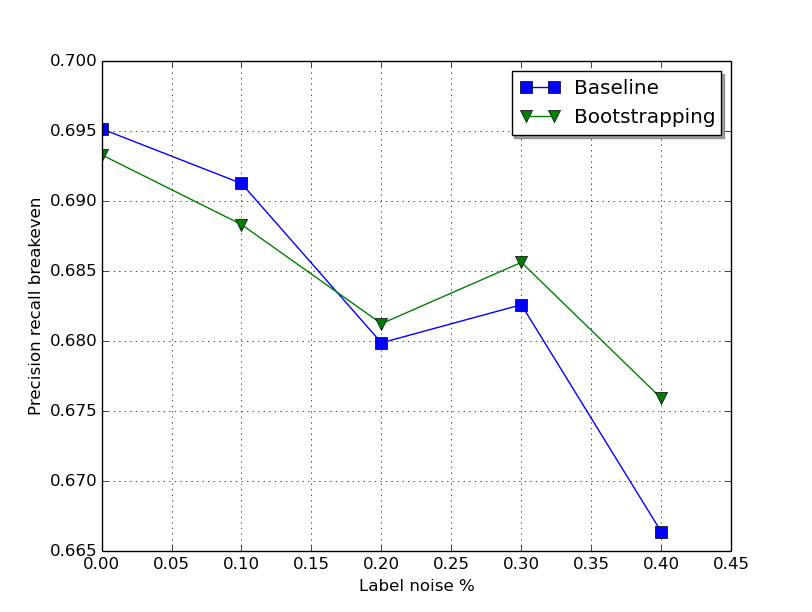
\includegraphics[width=\linewidth]{figs/E3/E3_pr_noise.png}
\caption{Precision and recall breakeven} \label{fig:E3_boot_mass_pr}
\end{subfigure}
\hspace*{\fill} % separation between the subfigures
\caption{E4 - Robustness of bootstrapping for increasing amount of label noise. Massachusetts Roads Dataset} \label{fig:E3_boot_mass}
\end{figure}

\begin{figure}
\begin{subfigure}{0.48\textwidth}
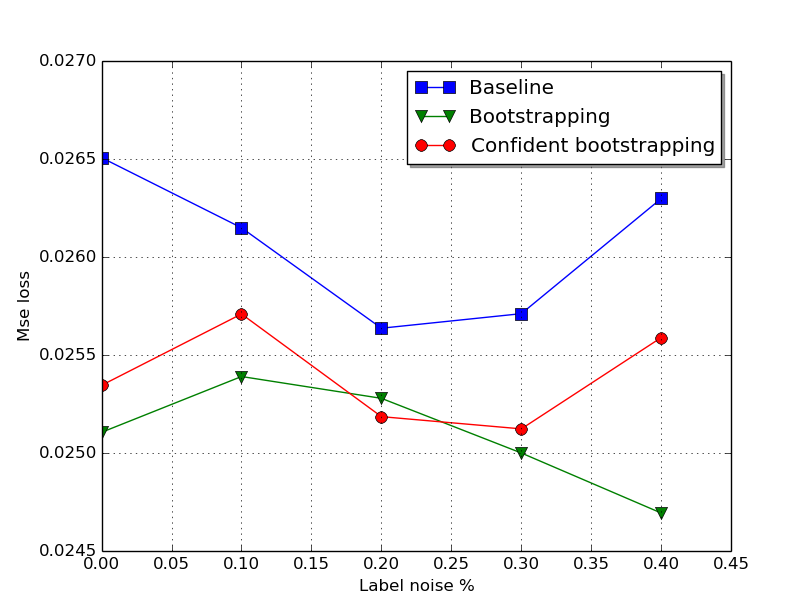
\includegraphics[width=\linewidth]{figs/E5/E5_lc_noise.png}
\caption{MSE test loss} \label{fig:E5_boot_norway_loss}
\end{subfigure}
\hspace*{\fill} % separation between the subfigures
\begin{subfigure}{0.48\textwidth}
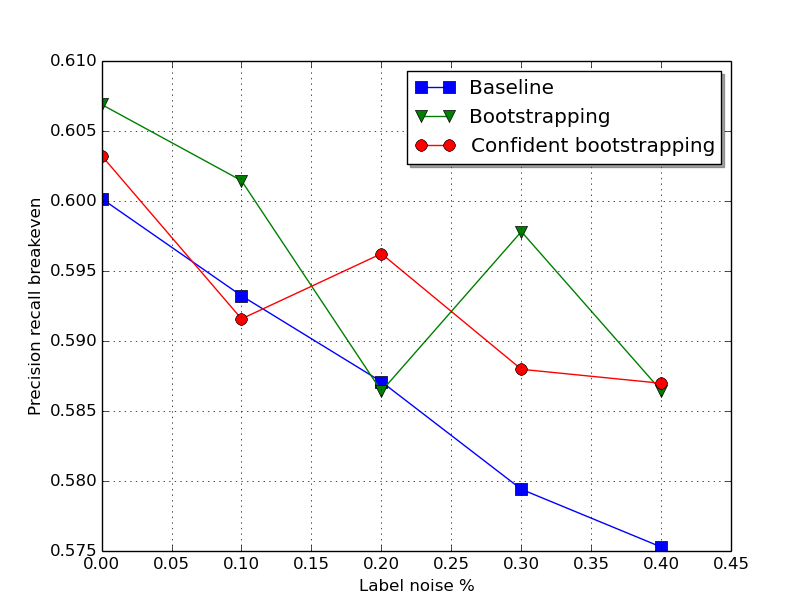
\includegraphics[width=\linewidth]{figs/E5/E5_pr_noise.png}
\caption{Precision and recall breakeven} \label{fig:E5_boot_norway_pr}
\end{subfigure}
\hspace*{\fill} % separation between the subfigures
\caption{E3 - Robustness of bootstrapping for increasing amount of label noise. Norwegian Roads Dataset} \label{fig:E5_boot_norway}
\end{figure}

Figure \ref{fig:E3_boot_mass_loss} displays the averaged test loss at different levels of label noise, for Experiment E3 \todo{Bad}. The baseline, which utilizes the cross-entropy loss function, seems to generally increase in test loss as the noise level is increased. The bootstrapping loss function has a lower test loss for noise levels above 10 percent.\\

Figure \ref{fig:E3_boot_mass_pr}, which displays the precision and recall breakeven values at increasing levels of label noise, shows a trend of decreasing values.  For label noise levels above 20 percent, bootstrapping surpasses the baseline. Though, the difference in performance is small.\\

The same kind of label noise experiment was also conducted for the Norwegian Roads Dataset, and include an additional plot of the confident bootstrapping performance. In Figure \ref{fig:E5_boot_norway_loss}, the test loss for bootstrapping and confident bootstrapping are consistently lower than the baseline. As expected, the precision and recall breakeven points for the baseline, decrease with increasing levels of omission noise. This can be seen in Figure \ref{fig:E4_boot_norway_vbase_pr}. Although the bootstrapping methods behave a bit more erratic, they generally tend to decrease at a slower rate \todo{A bit hard to see, doncha think!}.\\

A slightly different approach has been taken for Experiment E4. The road detection system has in this experiment been trained with labels from the label set N50. This label set has a higher rate of omission and registration noise than the labels in Massachusetts Roads Dataset, for instance. The test set however, consists of labels originating from the Vbase label set, which is more accurate. The result from this experiment is displayed in Figure \ref{fig:E4_boot_norway_vbase}\\

The difference between bootstrapping and confident bootstrapping is evident in Figure \ref{fig:E4_boot_norway_vbase_loss}. After epoch 90, the factor $\beta$ is decreased in favour of the model predictions. The test loss of confident bootstrapping sees an immediate decrease compared to the baseline, whereas the bootstrapping test loss increase in value. In terms of test loss, the confident bootstrapping loss function performed comparably to the baseline loss function, while the regular bootstrapping loss function performed worse. However, this result is not evident from the precision and recall curve, displayed in Figure \ref{fig:E4_boot_norway_vbase_pr}. In fact, the precision and recall breakeven values slightly favours the bootstrapping methods. This contradictory results between the MSE loss and the breakeven point, might be the result of the relaxed measure of precision, which ignores small misalignments between the prediction and label pixels.\\

\begin{figure}
\begin{subfigure}{0.48\textwidth}
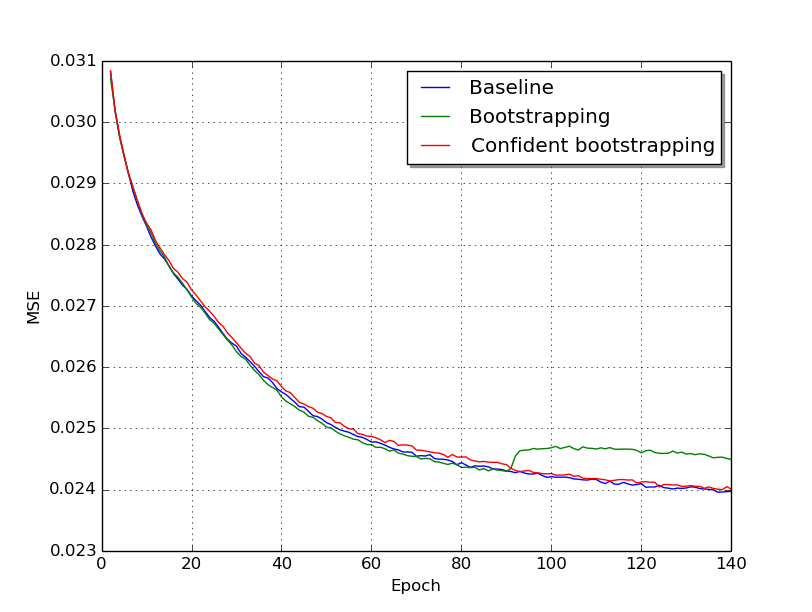
\includegraphics[width=\linewidth]{figs/E4/E4_lc.png}
\caption{MSE test loss} \label{fig:E4_boot_norway_vbase_loss}
\end{subfigure}
\hspace*{\fill} % separation between the subfigures
\begin{subfigure}{0.48\textwidth}
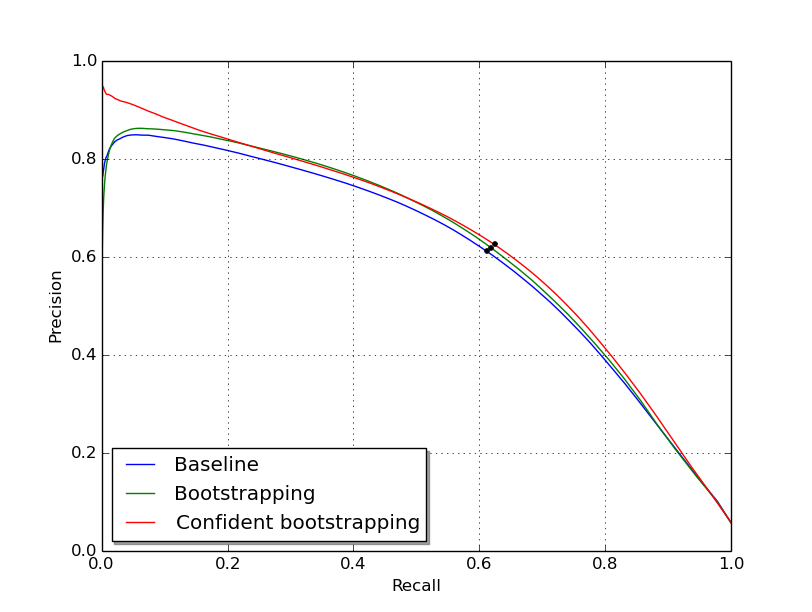
\includegraphics[width=\linewidth]{figs/E4/E4_pr.png}
\caption{Precision and recall comparison.} \label{fig:E4_boot_norway_vbase_pr}
\end{subfigure}
\hspace*{\fill} % separation between the subfigures
\caption{E4 - Comparison of loss functions for Norwegian Roads Dataset Vbase. The training set consists of labels with omission noise, and severe levels registration noise.} \label{fig:E4_boot_norway_vbase}
\end{figure}


\subsection{Road Detection System}
\label{sec:results_road_detection_system}
In this section, the road detection system was trained on a much larger patch dataset than in previous sections. In order for the patch dataset to fit in main memory, the examples were split into 9 separate stages each containing 442800 training examples. The content of the training set was switched during training. These switches are noticeable in the training loss plot in Figure \ref{fig:E6_performance_mass_lc}, where the loss increases slightly after a training set switch. The network converged to a \ac{MSE} test loss of 0.0232. \\

In Figure \ref{fig:E6_performance_mass_pr}, the averaged precision and recall curve is displayed. The precision and recall breakeven point for the system is 0.8341. Comparable experiments conducted in other works, are listed in Table \ref{tab:results_curriculum_learning_breakeven}.\todo{Footnote for other works. Unclear if averaged or not}\\

\begin{figure}
\begin{subfigure}{0.48\textwidth}
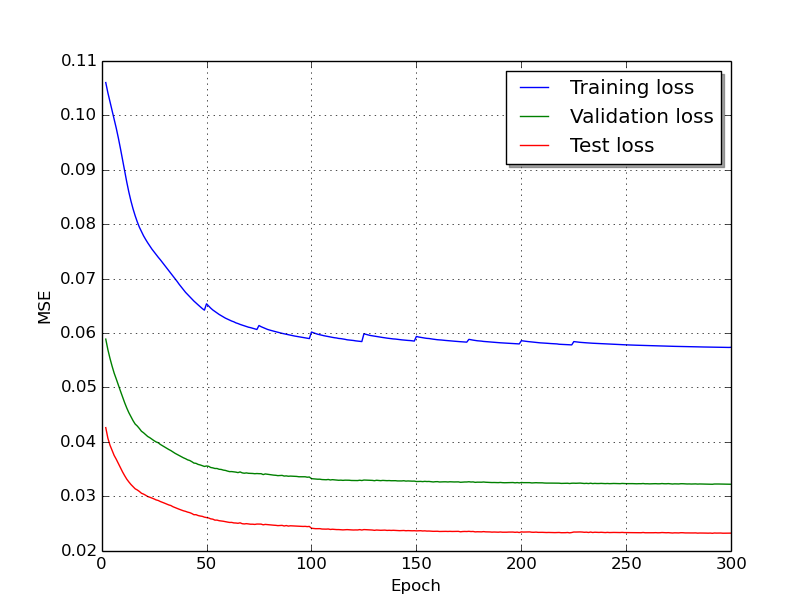
\includegraphics[width=\linewidth]{figs/E6/E6_lc_loss.png}
\caption{MSE loss} \label{fig:E6_performance_mass_lc}
\end{subfigure}
\hspace*{\fill} % separation between the subfigures
\begin{subfigure}{0.48\textwidth}
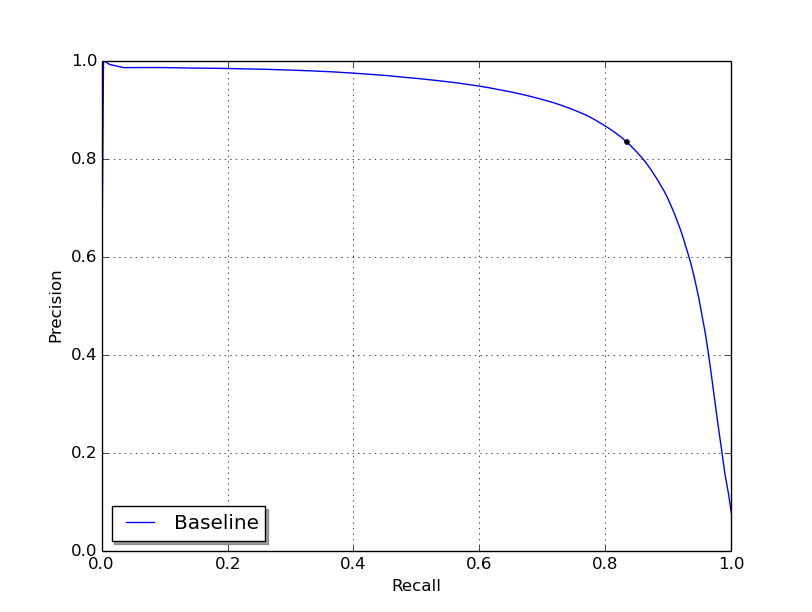
\includegraphics[width=\linewidth]{figs/E6/E6_pr.png}
\caption{Precision and recall.} \label{fig:E6_performance_mass_pr}
\end{subfigure}
\hspace*{\fill} % separation between the subfigures
\caption{E6 - Performance of road detection system trained with Massachusetts Roads Dataset.} \label{fig:E6_performance_mass}
\end{figure}

\begin{table}
\caption{Road detection system results.}
\begin{center}
\begin{adjustbox}{max width=\textwidth}
\begin{tabular}{+l ^r ^r}\hline
\rowstyle{\bfseries}
  System & breakeven & best network\\\hline
  Road detection system & 0.8341 & 0.84131\\
  Curriculum	 trained system &  & 0.863--\\
  \cite{MnihThesis} & 0.8873 & \\
  \cite{saito_building_and_roads} & 0.8866& \\\hline
\end{tabular}
\end{adjustbox}
\end{center}
\label{tab:results_curriculum_learning_breakeven}
\end{table}